
\begin{figure}[h!]
	\centering
	\tikzset{every picture/.style={line width=0.75pt}} %set default line width to 0.75pt        
	
	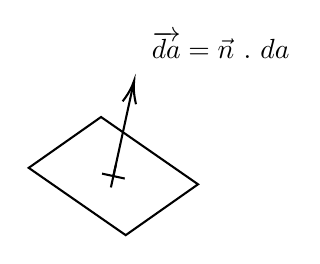
\begin{tikzpicture}[x=0.75pt,y=0.75pt,yscale=-1,xscale=1]
		%uncomment if require: \path (0,300); %set diagram left start at 0, and has height of 300
		
		%Flowchart: Data [id:dp7886171984971329] 
		\draw   (233.06,82.54) -- (279.79,114.96) -- (244.94,139.46) -- (198.21,107.04) -- cycle ;
		%Straight Lines [id:da19634912279776984] 
		\draw    (239,111) -- (248.58,66.95) ;
		\draw [shift={(249,65)}, rotate = 102.26] [color={rgb, 255:red, 0; green, 0; blue, 0 }  ][line width=0.75]    (10.93,-3.29) .. controls (6.95,-1.4) and (3.31,-0.3) .. (0,0) .. controls (3.31,0.3) and (6.95,1.4) .. (10.93,3.29)   ;
		\draw [shift={(239,111)}, rotate = 282.26] [color={rgb, 255:red, 0; green, 0; blue, 0 }  ][line width=0.75]    (-5.59,0) -- (5.59,0)(0,5.59) -- (0,-5.59)   ;
		
		% Text Node
		\draw (256,40) node [anchor=north west][inner sep=0.75pt]   [align=left] {$\displaystyle \overrightarrow{da} =\vec{n} \ .\ da$};
	\end{tikzpicture}
	\caption{The dot product $\protect\overrightarrow{\Phi}.\protect\overrightarrow{da}$ is the amount of particles passing through the infinitesimal cross section in unit time.}
	\label{fig_fluxCrossSection}
\end{figure}
